\chapter{Results}
\label{ch:results}

This chapter summarises the results published in the \NS\ technical
report~\cite{nvidia2026super}. The model is compared with two open models of
similar size: GPT-OSS-120B~\cite{openai2025gptoss} from OpenAI and
Qwen3.5-122B-A10B from Alibaba. Both are Mixture-of-Experts Transformers, so
the comparison isolates, as far as a comparison between different training
pipelines can, what the hybrid design contributes.

\section{Base Model}

Before any post-training, the pretrained base model is compared with two other
publicly available base models, Ling-flash-Base-2.0 and GLM-4.5-Air-Base
(Table~\ref{tab:base}). The \NS\ base model is the most accurate on almost
every task. The margins are largest on the harder reasoning benchmarks
(MMLU-Pro, GPQA-Diamond, MATH Level~5) and on long-context retrieval, where it
is the only one of the three evaluated beyond 128K tokens and still scores
71.0 on RULER at one million tokens.

\begin{table}[htbp]
\centering
\small
\caption[Base model comparison]{Base model comparison on selected benchmarks
(from~\cite{nvidia2026super}, Table~4). Best value in each row in bold.}
\label{tab:base}
\begin{tabular}{@{}lccc@{}}
\toprule
\textbf{Benchmark} & \textbf{\NS\ Base} & \textbf{Ling-flash-Base-2.0} & \textbf{GLM-4.5-Air-Base} \\
\midrule
MMLU & \textbf{86.01} & 81.00 & 81.00 \\
MMLU-Pro & \textbf{75.65} & 62.10 & 58.20 \\
GPQA-Diamond & \textbf{60.00} & 36.00 & 23.20 \\
GSM8K & 90.67 & \textbf{90.75} & 82.60 \\
MATH & \textbf{84.84} & 63.80 & 50.36 \\
MATH Level 5 & \textbf{70.00} & 39.80 & 26.30 \\
HumanEval & \textbf{79.40} & 70.10 & 76.30 \\
MBPP-Sanitized & \textbf{78.38} & 77.30 & 77.50 \\
WinoGrande & 78.93 & 78.37 & \textbf{83.82} \\
MGSM (multilingual) & \textbf{87.47} & 82.73 & 80.33 \\
RULER 64K & \textbf{92.26} & 72.12 & 80.26 \\
RULER 128K & \textbf{88.26} & 52.03 & 61.70 \\
RULER 1M & \textbf{71.00} & --- & --- \\
\bottomrule
\end{tabular}
\end{table}

\section{Post-Trained Model: Accuracy}

Figure~\ref{fig:headline} is the headline comparison from the report and
Table~\ref{tab:main} gives the numbers for a representative set of
benchmarks.

\begin{figure}[htbp]
  \centering
  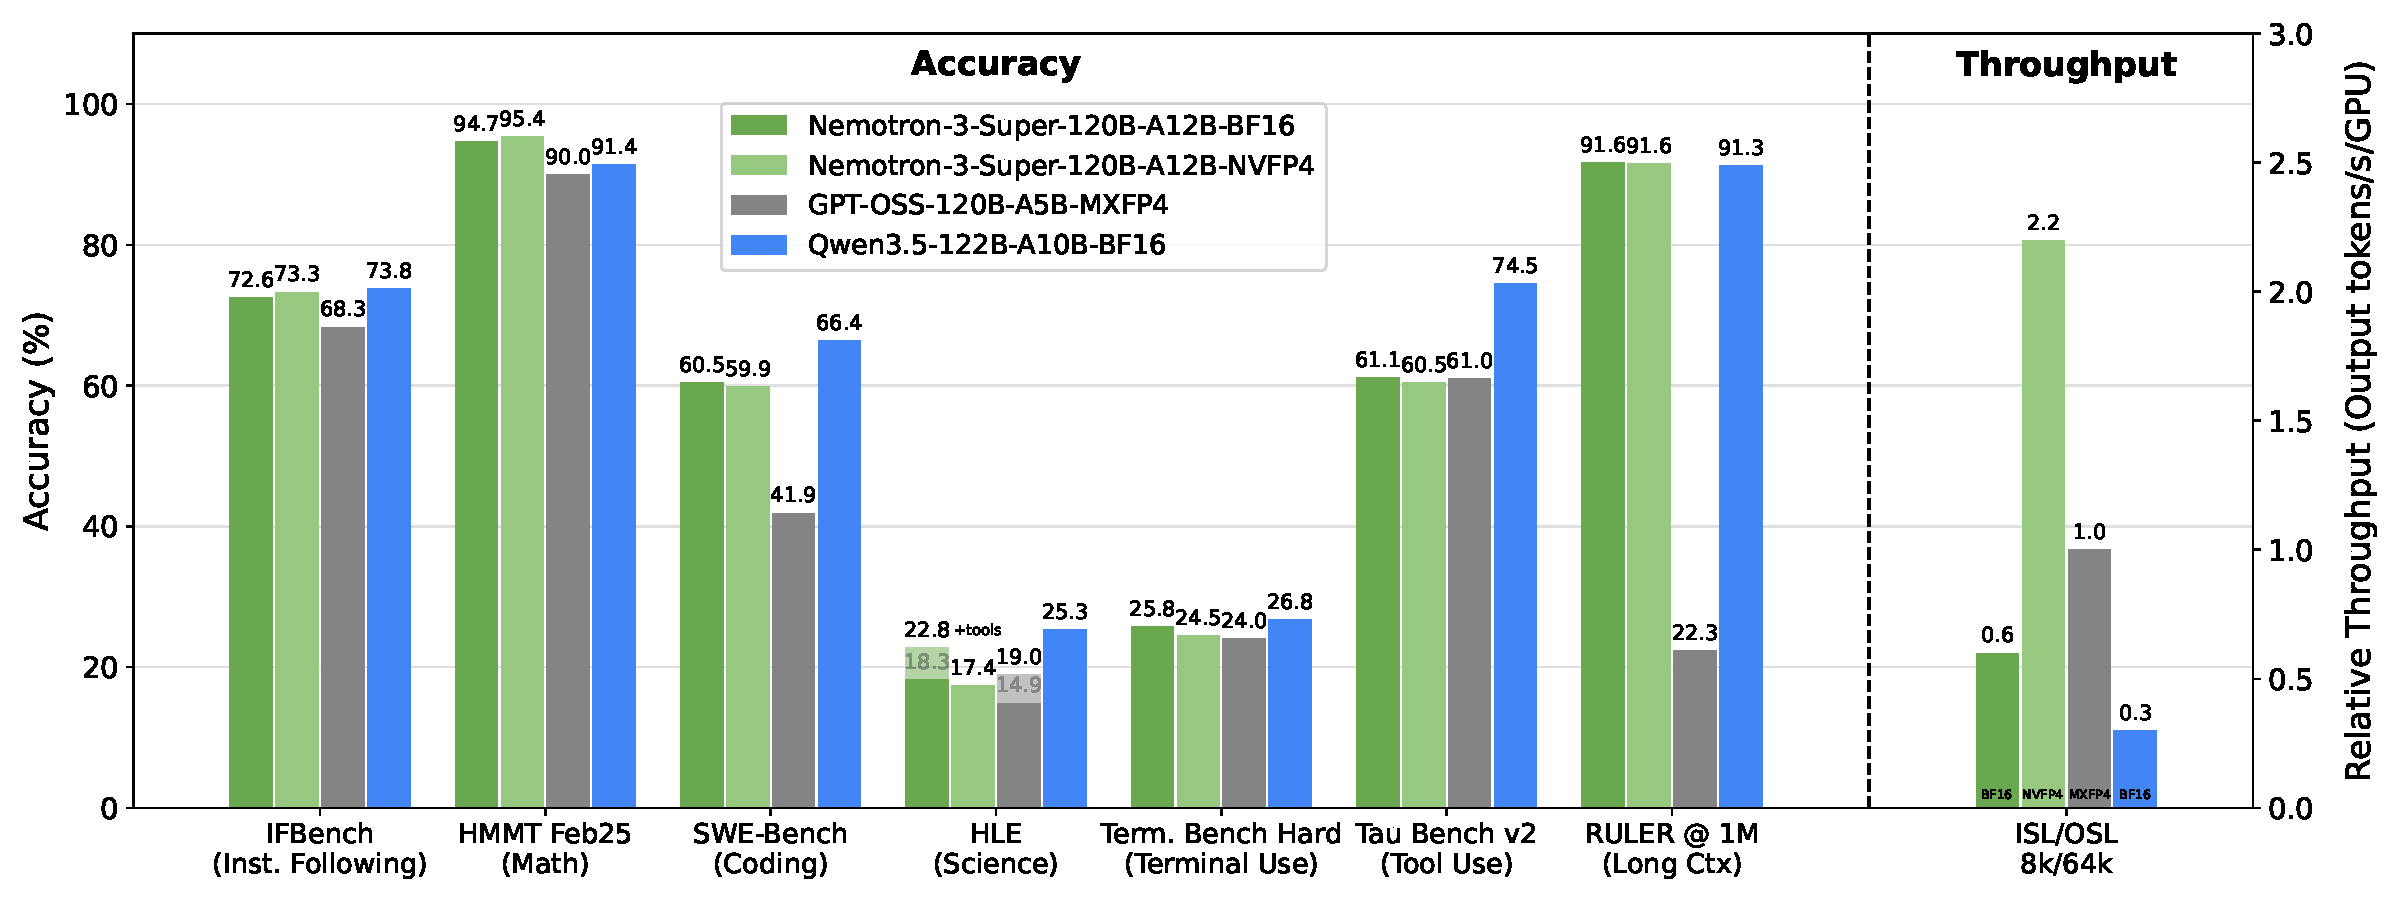
\includegraphics[width=\linewidth]{n3s-fig01-accuracy-throughput.pdf}
  \caption[Accuracy and throughput of Nemotron 3 Super against GPT-OSS-120B and Qwen3.5-122B]{Accuracy
  and throughput of \NS\ compared with GPT-OSS-120B and Qwen3.5-122B.
  Throughput is measured on B200 GPUs with 8k input and 64k output tokens.
  \source{NVIDIA (2026)~\cite{nvidia2026super}, Fig.~1}}
  \label{fig:headline}
\end{figure}

\begin{table}[htbp]
\centering
\small
\caption[Post-trained model comparison]{Post-trained \NS\ compared with
Qwen3.5-122B-A10B and GPT-OSS-120B on selected benchmarks
(from~\cite{nvidia2026super}, Table~5). Best value in each row in bold.}
\label{tab:main}
\begin{tabular}{@{}lccc@{}}
\toprule
\textbf{Benchmark} & \textbf{\NS} & \textbf{Qwen3.5-122B} & \textbf{GPT-OSS-120B} \\
\midrule
\multicolumn{4}{@{}l}{\emph{General knowledge and reasoning}} \\
MMLU-Pro & 83.73 & \textbf{86.70} & 81.00 \\
AIME25 (no tools) & 90.21 & 90.36 & \textbf{92.50} \\
HMMT Feb25 (no tools) & \textbf{93.67} & 91.40 & 90.00 \\
GPQA (no tools) & 79.23 & \textbf{86.60} & 80.10 \\
LiveCodeBench v5 & 81.19 & 78.93 & \textbf{88.00} \\
SciCode (subtask) & \textbf{42.05} & 42.00 & 39.00 \\
HLE (no tools) & 18.26 & \textbf{25.30} & 14.90 \\
\midrule
\multicolumn{4}{@{}l}{\emph{Agentic}} \\
Terminal Bench (hard subset) & 25.78 & \textbf{26.80} & 24.00 \\
Terminal Bench Core 2.0 & 31.00 & \textbf{37.50} & 18.70 \\
SWE-Bench (OpenHands) & 60.47 & \textbf{66.40} & 41.90 \\
TauBench V2 (average) & 61.15 & \textbf{74.53} & 61.00 \\
\midrule
\multicolumn{4}{@{}l}{\emph{Chat and instruction following}} \\
IFBench (prompt) & 72.56 & \textbf{73.77} & 68.32 \\
Arena-Hard-V2 & 73.88 & 75.15 & \textbf{90.26} \\
\midrule
\multicolumn{4}{@{}l}{\emph{Long context}} \\
AA-LCR & 58.31 & \textbf{66.90} & 51.00 \\
RULER 256k & \textbf{96.83} & 96.74 & 52.30 \\
RULER 512k & 95.22 & \textbf{95.95} & 46.70 \\
RULER 1M & \textbf{91.64} & 91.33 & 22.30 \\
\midrule
\multicolumn{4}{@{}l}{\emph{Multilingual}} \\
MMLU-ProX (average) & 79.36 & \textbf{85.06} & 76.59 \\
WMT24++ (en$\rightarrow$xx) & 86.67 & 87.84 & \textbf{88.89} \\
\bottomrule
\end{tabular}
\end{table}

Three observations can be made.

\textbf{Against GPT-OSS-120B.} \NS\ matches or beats GPT-OSS-120B on most of
the benchmarks listed. The lead is largest on agentic tasks---60.5 against
41.9 on SWE-Bench and 31.0 against 18.7 on Terminal Bench Core 2.0---which
reflects the emphasis on agentic data and RL environments during
post-training. GPT-OSS-120B remains ahead on a few benchmarks, notably
LiveCodeBench, AIME25 and Arena-Hard-V2.

\textbf{Against Qwen3.5-122B.} Qwen3.5-122B is the more accurate model on the
majority of rows: it leads on MMLU-Pro, GPQA, HLE, SWE-Bench, TauBench and
MMLU-ProX, in several cases by a clear margin. \NS\ is ahead on HMMT,
LiveCodeBench and RULER at 256k and 1M, and roughly level elsewhere. The
report itself describes the model as ``lagging behind Qwen-3.5-122B slightly''
on reasoning. The case for \NS\ over Qwen3.5 therefore rests on throughput
rather than on accuracy.

\textbf{Accuracy is ``comparable'', not uniformly better.} The fair summary is
that the hybrid model sits in the same accuracy class as the best open
Transformer MoE models of its size: ahead of one, somewhat behind the other.

\section{Long-Context Performance}

The clearest qualitative difference appears on RULER~\cite{hsieh2024ruler}, a
benchmark that measures how well a model actually uses a long context.
Figure~\ref{fig:ruler} plots the scores from Table~\ref{tab:main}. \NS\ loses
only about five points between 256k and one million tokens, finishing at
91.6. GPT-OSS-120B is already at 52.3 at 256k and falls to 22.3 at one million
tokens. Qwen3.5-122B, a Transformer, tracks \NS\ closely on this benchmark,
which shows that long-context \emph{accuracy} is not exclusive to hybrids;
what the hybrid changes is the \emph{cost} of serving such contexts.

\begin{figure}[htbp]
  \centering
  % RULER long-context accuracy, plotted from Table 5 of the Nemotron 3 Super report
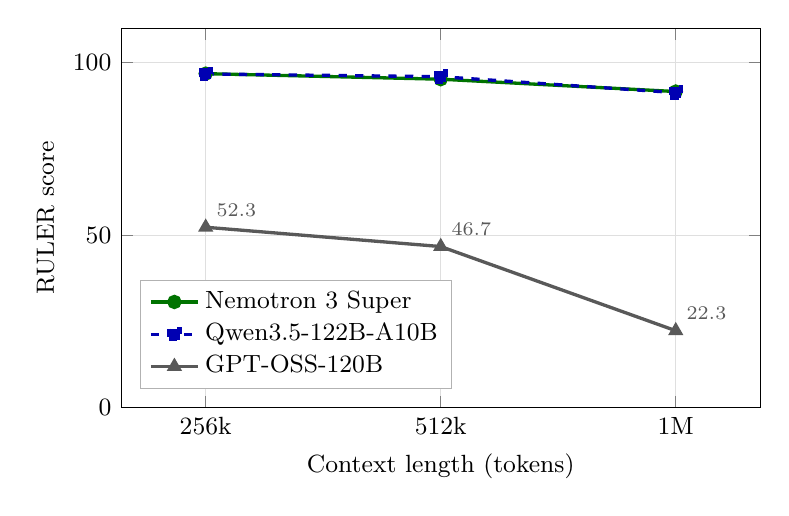
\begin{tikzpicture}
\begin{axis}[
  width=0.8\linewidth, height=6.4cm,
  symbolic x coords={256k,512k,1M}, xtick=data,
  xlabel={Context length (tokens)}, ylabel={RULER score},
  ymin=0, ymax=110, enlarge x limits=0.18,
  grid=major, grid style={gray!25},
  legend style={font=\small, at={(0.03,0.05)}, anchor=south west, draw=gray!60},
  legend cell align=left,
  tick label style={font=\small}, label style={font=\small},
  ]
\addplot[very thick, mark=*, green!45!black]
  coordinates {(256k,96.83) (512k,95.22) (1M,91.64)};
\addlegendentry{Nemotron 3 Super}
\addplot[very thick, mark=square*, blue!70!black, dashed]
  coordinates {(256k,96.74) (512k,95.95) (1M,91.33)};
\addlegendentry{Qwen3.5-122B-A10B}
\addplot[very thick, mark=triangle*, gray!70!black,
  nodes near coords, nodes near coords style={font=\scriptsize, anchor=south west}]
  coordinates {(256k,52.30) (512k,46.70) (1M,22.30)};
\addlegendentry{GPT-OSS-120B}
\end{axis}
\end{tikzpicture}

  \caption[RULER score against context length]{RULER score against context
  length for the three models (plotted by the author from the data
  in~\cite{nvidia2026super}, Table~5).}
  \label{fig:ruler}
\end{figure}

It is also notable that the score at one million tokens rose from 71.0 for the
base model (Table~\ref{tab:base}) to 91.6 after post-training, which included
long-context SFT data and a long-context RL environment.

\section{Inference Throughput}

Throughput is where the architecture pays off. On B200 GPUs, with 8k input
tokens and 64k output tokens---a setting typical of long reasoning or agentic
generation---\NS\ delivers up to 2.2$\times$ the throughput of GPT-OSS-120B
and up to 7.5$\times$ that of Qwen3.5-122B. Table~\ref{tab:throughput} lists
the relative values shown in Figure~\ref{fig:headline}.

\begin{table}[htbp]
\centering
\small
\caption[Relative inference throughput]{Relative inference throughput at 8k
input / 64k output tokens, normalised to GPT-OSS-120B (values read by the
author from~\cite{nvidia2026super}, Fig.~1)}
\label{tab:throughput}
\begin{tabular}{@{}llc@{}}
\toprule
\textbf{Model} & \textbf{Precision} & \textbf{Relative throughput} \\
\midrule
\NS\ 120B-A12B & NVFP4 & 2.2 \\
GPT-OSS-120B-A5B & MXFP4 & 1.0 \\
\NS\ 120B-A12B & BF16 & 0.6 \\
Qwen3.5-122B-A10B & BF16 & 0.3 \\
\bottomrule
\end{tabular}
\end{table}

Two details matter when reading these figures. First, the 2.2$\times$ result
belongs to the NVFP4 checkpoint; the unquantized BF16 checkpoint is slower
than the 4-bit GPT-OSS-120B. The headline speed is thus the product of the
architecture \emph{and} the quantization work of Chapter~\ref{ch:quant}, not
of the architecture alone. Second, at equal precision (BF16) \NS\ is about
twice as fast as Qwen3.5-122B even though it activates slightly more
parameters per token (12B against 10B). Here the difference does come from the
architecture: a long 64k-token generation is exactly the regime in which a
constant-size Mamba state beats a growing KV cache.

\section{Summary of Results}

\begin{itemize}
  \item The base model outperforms comparable public base models on nearly all
        benchmarks.
  \item The post-trained model matches or beats GPT-OSS-120B on most tasks and
        trails Qwen3.5-122B on several reasoning and agentic benchmarks.
  \item On RULER at one million tokens it scores 91.6, against 22.3 for
        GPT-OSS-120B.
  \item It runs up to 2.2$\times$ faster than GPT-OSS-120B and up to
        7.5$\times$ faster than Qwen3.5-122B.
  \item Quantization to NVFP4 retains a median of 99.8\% of BF16 accuracy, and
        MTP yields an average acceptance length of 3.45 tokens.
\end{itemize}
